%!TeX root=../../tcc.tex

%% ------------------------------------------------------------------------- %%


\chapter{Ordenação cinética}\label{ch:ordenacao-cinetica}
Considere o seguinte problema cinético.
Dada uma coleção de $n$ pontos em movimento retilíneo, o objetivo é responder consultas do tipo:
para um certo $i$, com $1 \leq i \leq n$, quem é o $i$-ésimo maior valor da coleção no instante corrente.

% Cada par $(x_0, v)$ representa um valor que está mudando linearmente
% com o tempo. Num instante arbitrário $t \geq 0$, o valor
% correspondente ao par $(x_0, v)$ é $x_0 + tv$.

Por exemplo, se tivermos quatro elementos na coleção, digamos
$\left(6, -\frac{1}{2}\right)$, $(5, 0)$, $\left(3,
\frac{1}{4}\right)$ e $\left(0, \frac{4}{3}\right)$, podemos
representar essa coleção como na Figura~\ref{fig:ordenacao:exemplo}.

\begin{figure}
    \centering
        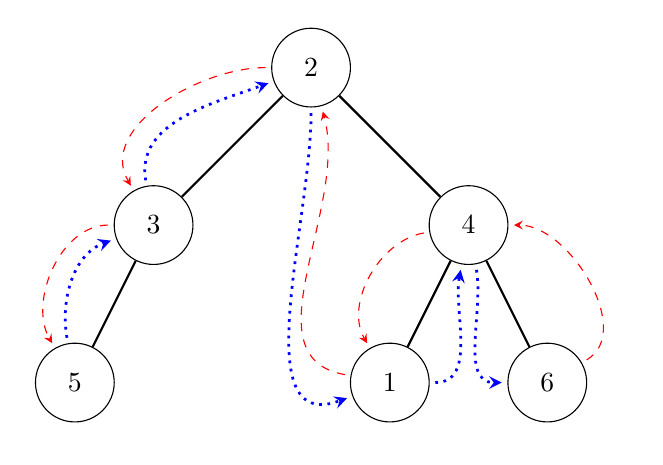
\begin{tikzpicture}[baseline=-2.25cm]
            \node[circle,draw,minimum size=1cm] (1) at (0,0)  {$2$};
            \node[circle,draw,minimum size=1cm] (2) at (-2,-2){$3$};
            \node[circle,draw,minimum size=1cm] (3) at (2,-2) {$4$};
            \node[circle,draw,minimum size=1cm] (4) at (-3,-4){$5$};
            \node[circle,draw,minimum size=1cm] (5) at (1,-4) {$1$};
            \node[circle,draw,minimum size=1cm] (6) at (3,-4) {$6$};
            % \node[label={7},circle,draw,minimum size=1cm] (7) at (3,-4) {$8$};
            % \node[label={8},circle,draw,minimum size=1cm] (8) at (-4,-6) {$4$};
            % \node[label={9},circle,draw,minimum size=1cm] (9) at (-2,-6) {$1$};
            \tikzstyle{filho}=[thick]
            \tikzstyle{pred}=[->, shorten >= 2pt, shorten <= 2pt,
                    dashed, >=stealth, red]
            \tikzstyle{sucessor}=[->, shorten >= 2pt, shorten <= 2pt,
                    dotted, >=stealth, blue, line width=0.35mm]
            % \tikzstyle{p4}=[->, shorten >= 2pt, shorten <= 2pt, dotted, >=stealth]
            \draw[filho] (1) -- (2);
            \draw[filho] (1) -- (3);
            \draw[filho] (2) -- (4);
            \draw[filho] (3) -- (5);
            \draw[filho] (3) -- (6);
            \draw[pred] (6) edge[out=30,in=0] (3);
            \draw[sucessor] (3) edge[out=280,in=180] (6);
            \draw[pred] (3) edge[out=190,in=120] (5);
            \draw[sucessor] (5) edge[out=0,in=260] (3);
            \draw[pred] (5) edge[out=170,in=285] (1);
            \draw[sucessor] (1) edge[out=270,in=200] (5);
            \draw[pred] (1) edge[out=180,in=120] (2);
            \draw[sucessor] (2) edge[out=100,in=200] (1);
            \draw[pred] (2) edge[out=180,in=120] (4);
            \draw[sucessor] (4) edge[out=100,in=200] (2);
        \end{tikzpicture}
        \qquad
        \qquad
        \qquad
        \begin{tabular}{|c|c|}
            \hline
            $i$ & $x_0$ \\
            \hline
            $1$ & $6$ \\

            $2$ & $3$ \\

            $3$ & $2$ \\

            $4$ & $7$ \\

            $5$ & $-2$ \\

            $6$ & $14$ \\
            \hline
        \end{tabular}
        \caption[Exemplo de estrutura da ABB]{Exemplo de árvore em
            que a ordem dos elementos, do menor para o maior no
            instante $\now = 0$, é $5 - 3 - 2 - 1 - 4 - 6$. Os
            apontadores para o elemento anterior são representados
            pelas setas vermelhas tracejadas e os apontadores para o
            elemento posterior são representados pelas setas azuis
            pontilhadas.}\label{fig:abb:exemplo}
\end{figure}

\newpage

Queremos dar suporte às seguintes operações:
\begin{itemize}
    \item \textsc{advance}$(t)$ $\rightarrow$ avança o tempo
    corrente para $t$;
    \item \textsc{change}$(j, v)$ $\rightarrow$ altera a
    velocidade do elemento $j$ para $v$;
    \item \textsc{query\_kth}$(i)$ $\rightarrow$ devolve o
    elemento cujo valor é o $i$-ésimo maior no instante atual.
\end{itemize}

%!TeX root=../ordenacao.tex

%% ------------------------------------------------------------------------- %%

\section{Lista Ordenada Cinética}
\label{lista:secao}
Um jeito natural de resolver o problema da lista ordenada cinética é
manter um vetor com os elementos da lista em ordem decrescente do
valor no instante atual.

Inicialmente o vetor começa com os valores dos elementos no instante
$t = 0$, ou seja, com o valor $x_0$ de cada elemento, e este vetor é
ordenado em ordem decrescente. Na verdade, o vetor pode armazenar
não os valores, mas os índices dos elementos, e fazemos ordenação
indireta. No caso de empates nos valores dos elementos, o desempate
será feito pela velocidade, ou seja, se dois elementos, digamos $i$
e $j$, possuem o mesmo valor $x_0$, mas a velocidade de $i$ é maior
que a de $j$, então $i$ será tratado como se possuísse maior valor
que $j$ no instante inicial. Esse mesmo critério de desempate será
aplicado em todos os instantes e também em todos os problemas daqui
em diante.

Uma vez de posse do vetor ordenado com os valores iniciais
decrescentemente, construímos um certificado para cada par de
elementos consecutivos no vetor. O $i$-ésimo certificado, denotado
pelo par $(i, t)$, se refere ao par das posições $i$ e $i + 1$. O
valor $t$ consiste no instante de tempo em que o $i$-ésimo elemento
deixará de ter um valor maior que o valor do $(i + 1)$-ésimo
elemento do vetor, se esse instante for maior ou igual a 0, ou em
geral ao instante atual. Do contrário, o valor $t$ consiste em
$+\infty$. O valor $t$ do certificado é o seu \underline{prazo de
validade}.

Esses prazos de validade determinam os \underline{eventos} que
potencialmente causarão modificações no vetor que mantém os
elementos ordenados pelo seu valor e consequentemente em alguns
certificados.

Esses $n - 1$ certificados são colocados em uma fila com
prioridades, com o prazo de validade determinando a prioridade.
Estamos interessados nos certificados com menor prazo de validade.
Ou seja, a fila com prioridades pode ser implementada com um heap de
mínimo que usa os prazos de validade como chave.

Para descrever a implementação das três operações, precisamos
estabelecer o nome das variáveis usadas. São elas:
\begin{enumerate}
    \item $n$: o número de elementos dados;
    \item $x_0$ e \textit{speed}: vetores com o valor e a
    velocidade inicial de cada um dos $n$ elementos;
    \item \now: instante atual;
    \item \textit{sorted}: vetor com os índices dos $n$
    elementos em ordem decrescente do seu valor no instante
    \textit{now};
    \item \textit{indS}: vetor de $n$ posições; \textit{indS}[$i$]
    guarda a posição em \textit{sorted} do elemento $i$;
    \item \textit{cert}: vetor com os $n-1$ certificados;
    \textit{cert}$[i]$ guarda o certificado entre $\sorted[i]$ e
    ${\sorted[i+1]}$, para~$1~\leq~i~<~n$;
    \item \textit{Q}: fila com prioridades para os certificados.
\end{enumerate}

A interface da fila com prioridades que utilizaremos inclui as duas
seguintes operações:
\begin{enumerate}
    \item \textsc{minPQ}$(Q)$: devolve o certificado $(i, t)$
    com chave $t$ mínima em $Q$;
    \item \textsc{updatePQ}$(Q, i, t)$: altera a chave do
    $i$-ésimo certificado para $t$ e ajusta $Q$ de acordo.
\end{enumerate}
O vetor $\textit{indS}$ nos permite implementar a operação
\textsc{change} de maneira eficiente, pois, dado um elemento $j$,
precisamos saber a posição $i$ do elemento $j$ em $\sorted$ para
recalcular os certificados relacionados com a posição $i$.

Para implementar a operação \textsc{updatePQ}$(Q, i, t)$ em tempo
logarítmico no número de elementos na fila $Q$, é necessário
utilizar um vetor adicional \textit{indQ} que guarda em
\textit{indQ}$[i]$ a posição do $i$-ésimo certificado em $Q$.

Com isso, a operação \textsc{advance}$(t)$ segue uma ideia bem
simples: enquanto $t$ for maior que o prazo de validade do próximo
evento, avançamos \textit{now} para esse prazo de validade e
tratamos esse evento. Nos problemas seguintes, a operação
\textsc{advance}$(t)$ será sempre a mesma; as únicas mudanças
ocorrerão no tratamento de um evento. Um evento está associado a um
certificado $(i, t)$ que expira quando $\now = t$. O tratamento do
evento correspondente ao certificado $(i, t)$ consiste em trocar de
lugar os índices das posições $i$ e $i + 1$ do vetor
\textit{sorted}, recalcular o prazo de validade do $(i-1)$-ésimo
certificado se $i > 1$, e do $(i + 1)$-ésimo certificado se $i < n -
1$. O $i$-ésimo certificado também deve ser ajustado para $+\infty$.
Finalmente, é necessário fazer ajustes em $Q$, alterando a chave dos
certificados que sofreram alteração.

\begin{algorithm}[H]
    \caption{Função \textsc{advance}.} \label{alg:lista-ordenada:advance}
\begin{algorithmic}[1]
    \Function{advance}{$t$}
        \If{$t < $ \now}
            \State \Return
        \EndIf
        \State $i \leftarrow \Call{minPQ}{$Q$}$
        \While{$t \geq$ \cert[$i$]}
            \State \now $~\leftarrow$ \cert[i]
            \State $\Call{event}$
            \State $i \leftarrow \Call{minPQ}{$Q$}$
        \EndWhile
        \State \now $~\leftarrow$ $t$
    \EndFunction
\end{algorithmic}
\end{algorithm}

Na implementação da operação \textsc{event}, utilizaremos a rotina
\textsc{update}$(i)$ para calcular a nova validade $t$ do $i$-ésimo
certificado, se $1 \leq i < n$, e fazer os devidos ajustes em $Q$.
Para calcular $t$, utilizaremos uma rotina chamada
\textsc{expire}$(i, j)$, que calcula a validade dos certificados
entre os elementos $i$ e $j$. A rotina auxiliar \textsc{expire}$(i,
j)$ não mudará para outros problemas, mantendo a mesma definição.

\begin{algorithm}[H]
    \caption{Função \textsc{update}.} \label{torneioi:update}
    \begin{algorithmic}[1]
        \Function{update}{$e$}
            \If{$e \neq$ NULL}
                \State $e'\leftarrow \torneio[(e.\lastmatch)/2]$
                \State $t \leftarrow $ \Call{expire}{$e, e'$}
                \State \Call{updatePQ}{$Q,e,t$}
            \EndIf
        \EndFunction
        % \LineComment{Em expire$(e, e')$, $e'$ pode ser nulo e
        % nesse caso o retorno é $+\infty$.}
        % \LineComment{\Call{expire}{$e,e'$} calcula a validade do
        % certificado entre os elementos $e$ e $e'$, se $e'$ é NULL
        % retorna $+\infty$}
    \end{algorithmic}
\end{algorithm}

\begin{algorithm}[H]
    \caption{Função \textsc{event}.} \label{torneioi:evento}
    \begin{algorithmic}[1]
        \Function{event}{\nnull}
            \State $e \leftarrow  $ \Call{minPQ}{$Q$}
            \While{$e.\cert$ = \now}
                \State $j \leftarrow e.\lastmatch$
                \State $k \leftarrow 2\cdot \floor{\frac{j}{2}}
                + ((j + 1)\mod2)$ \Comment{adversário}
                \While{$j > 1$ \AND \Call{value}{$j$} $\geq$
                    \Call{value}{$k$}}
                    \State \torneio[$\floor{\frac{j}{2}}$]
                    $\leftarrow~$\torneio[$j$]
                    \State $\torneio[k].\lastmatch$ $\leftarrow k$
                    \State \Call{update}{$\torneio[k]$}
                    \State $j \leftarrow \floor{\frac{j}{2}}$
                    \State $k \leftarrow 2\cdot \floor{\frac{j}{2}}
                    + ((j + 1)\mod2)$ \Comment{adversário}
                \EndWhile
                \State $\torneio[j].\lastmatch \leftarrow j$
                \State \Call{update}{$\torneio[j]$}
                \State $e \leftarrow  $ \Call{minPQ}{$Q$}
            \EndWhile
        % \LineComment{swapHeap$(i, \floor{\frac{i}{2}})$ troca \heap[$i$] por \heap$\left[\floor{\frac{i}{2}}\right]$}
        \EndFunction
%        \LineComment{\Call{compare}{$i, j$} retorna se o valor
%        de $i$ é maior que o valor de $j$.}
    \end{algorithmic}
\end{algorithm}

As figuras \ref{fig:lista:expire} e \ref{fig:lista:update} ilustram
o tratamento do evento de expiração do segundo certificado.

\begin{figure}[H]
    \centering
    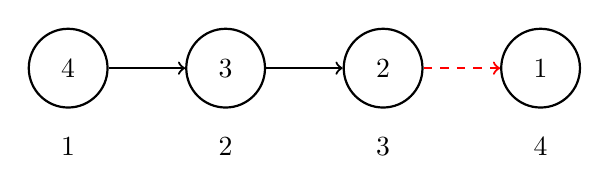
\begin{tikzpicture}[thick]
        \edef\pos{0}
        \foreach \x in {1, 2,..., 4}{
            \pgfmathparse{\pos+2}
            \xdef\pos{\pgfmathresult}
            \node  at (\pos, -1) {$\x$};
        }
        \node[circle,draw, minimum size=1cm] (1) at  (2, 0) {$4$};
        \node[circle,draw, minimum size=1cm] (2) at  (4, 0) {$3$};
        \node[circle,draw, minimum size=1cm] (3) at  (6, 0) {$2$};
        \node[circle,draw, minimum size=1cm] (4) at  (8, 0) {$1$};
        \draw[->] (1) -- (2);
        \draw[->] (2) -- (3);
        \draw[->, color=red, dashed] (3) -- (4);
    \end{tikzpicture}
    \caption[Exemplo de expiração de certificado da lista ordenada]{No exemplo da
    Figura~\ref{fig:ordenacao:exemplo}, \cert[3] expirou no instante $t = 2$.}
    \label{fig:lista:expire}
\end{figure}

\begin{algorithm}[H]
    \caption{Função \textsc{update}.} \label{torneioi:update}
    \begin{algorithmic}[1]
        \Function{update}{$e$}
            \If{$e \neq$ NULL}
                \State $e'\leftarrow \torneio[(e.\lastmatch)/2]$
                \State $t \leftarrow $ \Call{expire}{$e, e'$}
                \State \Call{updatePQ}{$Q,e,t$}
            \EndIf
        \EndFunction
        % \LineComment{Em expire$(e, e')$, $e'$ pode ser nulo e
        % nesse caso o retorno é $+\infty$.}
        % \LineComment{\Call{expire}{$e,e'$} calcula a validade do
        % certificado entre os elementos $e$ e $e'$, se $e'$ é NULL
        % retorna $+\infty$}
    \end{algorithmic}
\end{algorithm}

\begin{algorithm}
    \caption{Função \textsc{query\_kth}.} \label{abb:query}
\begin{algorithmic}[1]
    \Function{query\_kth}{$i$}
        \State $node \leftarrow root$
        \State $r \leftarrow \Call{rsize}{node}$
        \While{$i \neq r + 1$}
        \If{$i \leq r$}
            \State $node \leftarrow node.right$
        \Else
            \State $node \leftarrow node.left$
            \State $i \leftarrow i - (r + 1)$
        \EndIf
        \State $r \leftarrow \Call{rsize}{node}$
        \EndWhile
        \State \Return $node.key$
    \EndFunction
\end{algorithmic}
\end{algorithm}

\begin{algorithm}
    \caption{Função \textsc{change}.} \label{lista:change}
\begin{algorithmic}[1]
    \Function{change}{$j, v$}
        \State $x_0$[$j$] $\leftarrow  x_0$[$j$]
        $+~($\speed[$j$]$~-~v)~\cdot~$\now;
        \State \speed[$j$] $\leftarrow  v$
        \State $i \leftarrow$ \inds[$j$]
        \State \Call{update}{$i$}
        \State \Call{update}{$i - 1$}
    \EndFunction
\end{algorithmic}
\end{algorithm}

A operação \textsc{query\_kth}$(i)$ consiste em devolver
\textit{sorted}$[i]$, enquanto que a operação \textsc{change}$(j,
v)$ consiste em alterar a posição $x_0[j]$ para $x_0[j] +
(\mathit{speed}[j] - v)\cdot now$, a posição \textit{speed}[j] para
\textit{v} e recalcular os eventuais certificados de que $j$
participa. O novo valor da posição $x_0[j]$ corresponde à posição
inicial do elemento caso ele tivesse começado com essa velocidade e
estivesse na posição atual agora. Para tanto, a partir da posição
$i$ em que $j$ se encontra no vetor \textit{sorted}, podemos
recalcular \textit{cert}$[i - 1]$ se $i > 1$ e \textit{cert}$[i]$ se
$i < n$, como ilustrado na figura \ref{fig:lista:after}, acionando
a rotina \textsc{updatePQ} para fazer os devidos acertos em~$Q$
correspondentes a estas modificações.

\begin{figure}
    \centering
    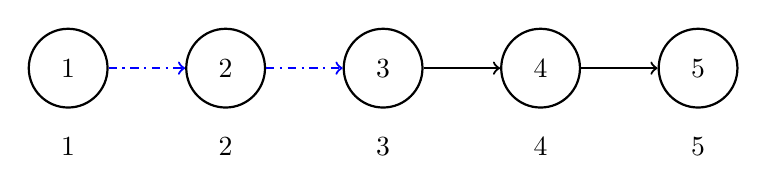
\begin{tikzpicture}[thick]
        \edef\pos{0}
        \foreach \x in {1, 2,..., 5}{
            \pgfmathparse{\pos+2}
            \xdef\pos{\pgfmathresult}
            \node[circle,draw, minimum size=1cm] (\x) at
                (\pos, 0) {$\x$};
            \node  at (\pos, -1) {$\x$};
        }
        % \foreach \x [evaluate=\x as \y using int(\x + 1)] in {1, 2,..., 4}{
        %     \ifthenelse{\x==2}{\draw[->, draw=red] (\x) -- (\y);}{\draw[->, draw=black] (\x) -- (\y);}
        % }
        \draw[->, color=blue, dashdotted] (1) -- (2);
        \draw[->, color=blue, dashdotted] (2) -- (3);
        \draw[->] (3) -- (4);
        \draw[->] (4) -- (5);
        % \draw[->] (1) edge (2) (2) edge (3) (3) edge (4) (4) edge (5)
    \end{tikzpicture}
    \caption[Certificados atualizados]{Após a mudança de velocidade
            do elemento 2, que se encontra em \sorted[2], \cert[1] e
            \cert[2] foram atualizados.}
    \label{fig:lista:after}
\end{figure}

%!TeX root=./ordenacao.tex


\section{Árvore binária balanceada de busca} \label{sec:abb}

Manter um vetor ordenado é uma boa maneira de resolver o problema da
lista ordenada cinética dando suporte às operações
\textsc{advance}$(t)$, \textsc{change}$(j,v)$ e
\textsc{query\_kth}$(i)$.
Poderíamos também querer dar suporte, além das operações citadas, às seguintes operações:

\begin{itemize}
    \item \textsc{insert}$(v, x_t) \rightarrow$ insere um
    elemento com velocidade $v$ e valor $x_t$ no instante \now;
    \item \textsc{delete}$(i) \rightarrow$ remove o elemento
    $i$ no instante \now.
\end{itemize}

Para inserir um elemento no vetor ordenado, antes teríamos de
encontrar a posição que este deveria ocupar no vetor.
Digamos que seja a posição $j$.
Após encontrar a posição, movemos todos os elementos, a partir da posição $j$, uma posição à
frente e colocamos o elemento na posição~$j$.
Após isso, os certificados de $j$~até~$n-1$ devem ser atualizados, pois esses elementos mudaram de
posição no vetor, e um novo certificado será criado, o $n$-ésimo
certificado.
Ademais, o total de elementos $n$ deve ser mudado para $n + 1$.
O novo certificado também deve ser inserido na fila com prioridades.

Só a operação de inserir um novo elemento no vetor já pode se tornar
pouco eficiente com uma grande quantidade de elementos sendo
inseridos no começo do vetor, consumindo tempo linear por inserção.
Como a remoção de um elemento no vetor ordenado envolve uma
sequência parecida de operações, da mesma maneira se torna pouco
eficiente, também consumindo tempo linear no pior caso.

Dessa forma, apesar da lista ordenada cinética implementada
manipulando um vetor ser uma estrutura eficiente para a operação
\textsc{query\_kth}$(i)$, com um consumo de tempo constante, o
consumo de tempo para as operações \textsc{insert}$(v, x_t)$ e
\textsc{delete}$(i)$ é, no pior caso, proporcional ao número de
elementos, o que pode ser ruim para uma grande quantidade de
elementos, inserções e remoções.

Podemos equilibrar o consumo de tempo das operações
\textsc{query\_kth}$(i)$, \textsc{insert}$(v, x_t)$ e
\textsc{delete}$(i)$ em tempo logarítmico no número de elementos,
usando uma ABBB (árvore binária balanceada de busca).
Os pontos serão armazenados na ABBB tendo o seu valor no instante \now~como
chave.

Além da ABBB, para garantirmos a eficiência das operações
\textsc{event}, \textsc{change}, \textsc{insert} e \textsc{delete},
cada elemento terá um apontador para o seu predecessor e um
apontador para o seu sucessor, formando uma lista duplamente ligada
ordenada pelo valor do elemento no instante \now; veja a Figura~\ref{fig:abb:exemplo}.

\begin{figure}
    \centering
        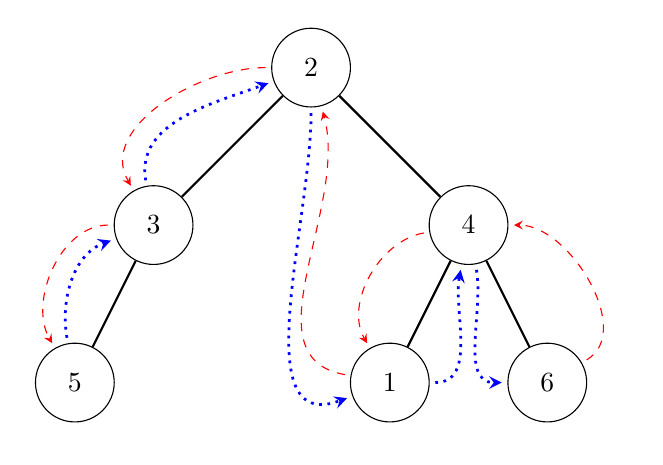
\begin{tikzpicture}[baseline=-2.25cm]
            \node[circle,draw,minimum size=1cm] (1) at (0,0)  {$2$};
            \node[circle,draw,minimum size=1cm] (2) at (-2,-2){$3$};
            \node[circle,draw,minimum size=1cm] (3) at (2,-2) {$4$};
            \node[circle,draw,minimum size=1cm] (4) at (-3,-4){$5$};
            \node[circle,draw,minimum size=1cm] (5) at (1,-4) {$1$};
            \node[circle,draw,minimum size=1cm] (6) at (3,-4) {$6$};
            % \node[label={7},circle,draw,minimum size=1cm] (7) at (3,-4) {$8$};
            % \node[label={8},circle,draw,minimum size=1cm] (8) at (-4,-6) {$4$};
            % \node[label={9},circle,draw,minimum size=1cm] (9) at (-2,-6) {$1$};
            \tikzstyle{filho}=[thick]
            \tikzstyle{pred}=[->, shorten >= 2pt, shorten <= 2pt,
                    dashed, >=stealth, red]
            \tikzstyle{sucessor}=[->, shorten >= 2pt, shorten <= 2pt,
                    dotted, >=stealth, blue, line width=0.35mm]
            % \tikzstyle{p4}=[->, shorten >= 2pt, shorten <= 2pt, dotted, >=stealth]
            \draw[filho] (1) -- (2);
            \draw[filho] (1) -- (3);
            \draw[filho] (2) -- (4);
            \draw[filho] (3) -- (5);
            \draw[filho] (3) -- (6);
            \draw[pred] (6) edge[out=30,in=0] (3);
            \draw[sucessor] (3) edge[out=280,in=180] (6);
            \draw[pred] (3) edge[out=190,in=120] (5);
            \draw[sucessor] (5) edge[out=0,in=260] (3);
            \draw[pred] (5) edge[out=170,in=285] (1);
            \draw[sucessor] (1) edge[out=270,in=200] (5);
            \draw[pred] (1) edge[out=180,in=120] (2);
            \draw[sucessor] (2) edge[out=100,in=200] (1);
            \draw[pred] (2) edge[out=180,in=120] (4);
            \draw[sucessor] (4) edge[out=100,in=200] (2);
        \end{tikzpicture}
        \qquad
        \qquad
        \qquad
        \begin{tabular}{|c|c|}
            \hline
            $i$ & $x_0$ \\
            \hline
            $1$ & $6$ \\

            $2$ & $3$ \\

            $3$ & $2$ \\

            $4$ & $7$ \\

            $5$ & $-2$ \\

            $6$ & $14$ \\
            \hline
        \end{tabular}
        \caption[Exemplo de estrutura da ABB]{Exemplo de árvore em
            que a ordem dos elementos, do menor para o maior no
            instante $\now = 0$, é $5 - 3 - 2 - 1 - 4 - 6$. Os
            apontadores para o elemento anterior são representados
            pelas setas vermelhas tracejadas e os apontadores para o
            elemento posterior são representados pelas setas azuis
            pontilhadas.}\label{fig:abb:exemplo}
\end{figure}

No que diz respeito aos certificados, antes um certificado estava
associado a uma posição e, no vetor, ao inserirmos um elemento em
uma determinada posição, teríamos que deslocar % que atualizar
todos os certificados conseguintes àquela posição.
Agora, para que consigamos alterar apenas uma quantidade constante de certificados
após uma inserção, os certificados não estarão mais associados a uma
posição e sim aos elementos.

O certificado $i$ se refere à relação estabelecida entre o elemento
$i$ e seu predecessor e consiste no instante de tempo em que o
elemento $i$ deixará de ter um valor maior que o valor do seu
predecessor, se esse instante for maior que o instante atual.
Do contrário, o certificado consiste em $+\infty$.
Se o elemento $i$ não possui predecessor, então o certificado também consiste em
$+\infty$.
Veja a Figura~\ref{fig:abb:cert}.

\begin{figure}
    \centering
    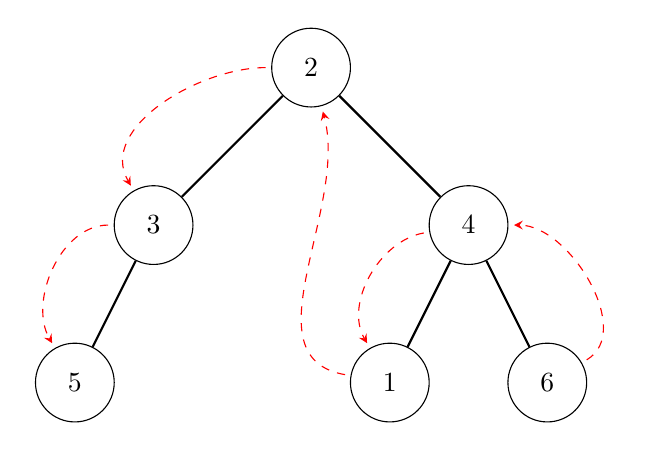
\begin{tikzpicture}[baseline=-2.25cm]
        \node[circle,draw,minimum size=1cm] (1) at (0,0)  {$2$};
        \node[circle,draw,minimum size=1cm] (2) at (-2,-2){$3$};
        \node[circle,draw,minimum size=1cm] (3) at (2,-2) {$4$};
        \node[circle,draw,minimum size=1cm] (4) at (-3,-4){$5$};
        \node[circle,draw,minimum size=1cm] (5) at (1,-4) {$1$};
        \node[circle,draw,minimum size=1cm] (6) at (3,-4) {$6$};
        \tikzstyle{filho}=[thick]
        \tikzstyle{pred}=[->, shorten >= 2pt, shorten <= 2pt,
            dashed, >=stealth, red]
        \tikzstyle{sucessor}=[->, shorten >= 2pt, shorten <= 2pt,
            dotted, >=stealth, line width=0.35mm]
        \draw[filho] (1) -- (2);
        \draw[filho] (1) -- (3);
        \draw[filho] (2) -- (4);
        \draw[filho] (3) -- (5);
        \draw[filho] (3) -- (6);
        \draw[pred] (6) edge[out=30,in=0] (3);
        \draw[pred] (3) edge[out=190,in=120] (5);
        \draw[pred] (5) edge[out=170,in=285] (1);
        \draw[pred] (1) edge[out=180,in=120] (2);
        \draw[pred] (2) edge[out=180,in=120] (4);
    \end{tikzpicture}
    \qquad
    \qquad
    \qquad
    \begin{tabular}{|c|c|c|c|}
        \hline
        $i$ & $x_0$ & $v$ & $\cert[i]$ \\
        \hline
        $1$ & $6$ & $2$ & $1$ \\

        $2$ & $3$ & $5$ & $+\infty$ \\

        $3$ & $2$ & $1$ & $2$ \\

        $4$ & $7$ & $4$ & $+\infty$ \\

        $5$ & $-2$ & $3$ & $+\infty$ \\

        $6$ & $14$ & $0.5$ & $2$ \\
        \hline
    \end{tabular}
    \caption[Representação dos certificados da ABB]{Certificados
            representados pelas setas vermelhas tracejadas. O
            certificado do elemento $5$ vale $+\infty$.}
            \label{fig:abb:cert}
\end{figure}

Esses $n$ certificados também serão colocados em uma fila com
prioridades, com o prazo de validade determinando a prioridade.
A fila com prioridades agora também deverá suportar operações
como a inserção e remoção de certificados.

Para descrever as implementações das operações, vamos
estabelecer os nomes dos objetos, variáveis e rotinas
auxiliares utilizados:
\begin{enumerate}
    \item $n$: número de elementos no instante \now;
    \item \no: objeto que compõe a árvore binária balanceada
    de busca, com atributos:
    \begin{enumerate}
        \item \esq$:$ aponta para a raiz da subárvore
        esquerda do nó;
        \item \dir$:$ aponta para a raiz da subárvore
        direita do nó;
        \item \textit{key}$:$ aponta para um elemento;
        \item \children$:$ quantidade de nós que a subárvore
        enraizada neste nó possui.
        Este atributo será importante para a operação \textsc{query\_kth}$(i)$;
    \end{enumerate}
    \item \raiz: nó que é a raiz da árvore binária balanceada de
    busca;
    \item \elemento: objeto com os seguintes atributos:
    \begin{enumerate}
        \item \id: vem de \textit{identifier} e é o atributo
        para identificar o objeto.
        Assim, daqui em diante, usaremos elemento $i$ para nos
        referirmos ao elemento cujo \id~é $i$;
        \item \speed: velocidade do elemento;
        \item \initv: valor que o elemento possuía no
        instante~$t = 0$;
        \item \nex: apontador para o elemento imediatamente
        posterior a este na coleção, no instante \now.
        O elemento imediatamente posterior a $i$ é aquele
        que possui o menor valor dentre a coleção de
        elementos que possuem valor maior que o elemento
        $i$;
        \item \prev: apontador para o elemento imediatamente
        anterior a este na coleção, no instante \now;
        \item \pqpos: vem de \textit{priority queue position} e
        aponta para a posição do certificado associado
        ao elemento na fila com prioridades;
        \item \cert: vem de \textit{certificate} e é o prazo de
        validade do certificado entre este elemento e o elemento
        apontado por \prev; se \prev~não aponta para ninguém,
        \cert~vale $+\infty$;
        \item \no: apontador para o nó da árvore binária de busca em
        que o elemento se encontra;
    \end{enumerate}
    \item \Q: fila com prioridades que contém os elementos;
    o elemento com certificado de menor valor estará à frente da fila;

    \item \textsc{insertKey}$(\text{\raiz},e)\rightarrow$ insere
    $e$, um elemento, na árvore binária balanceada de busca com raiz
    \raiz~e retorna a, possivelmente nova, raiz da árvore.
    No processo também atualiza a lista ligada de elementos;

    \item \textsc{deleteKey}$(\text{\raiz},e)\rightarrow$ remove
    $e$, um elemento, da árvore binária balanceada de busca com raiz
    \raiz~e retorna a, possivelmente nova, raiz da árvore.
    No processo também atualiza a lista ligada de elementos.

\end{enumerate}
Para a implementação das operações \textsc{change}$(j, v)$ e
\textsc{delete}$(i)$, precisamos de alguma maneira recuperar um
elemento baseado no seu \id.
Para tal, podemos utilizar uma tabela de símbolos, implementada por uma árvore binária balanceada
de busca ou uma tabela de dispersão.
A seguir~estão três operações que nos ajudarão a recuperar os elementos:

\begin{enumerate}
    \item \textsc{getObject}$(i)\rightarrow$ retorna o elemento $i$;
    \item \textsc{insertObject}$(e) \rightarrow$ insere $e$,
    que é um elemento, na estrutura;
    \item \textsc{deleteObject}$(e) \rightarrow$ remove $e$,
    que é um elemento, da estrutura.
\end{enumerate}

Para permitir a inserção e remoção de certificados, a interface da
fila com prioridades será reformulada, contando com duas operações
extras:

\begin{enumerate}
    \item \textsc{insertPQ}$(Q, e, t) \rightarrow$ insere $(e, t)$
    na fila com prioridades $Q$, sendo $t$ o prazo de validade do certificado de $e$;
    \item \textsc{deletePQ}$(Q, e) \rightarrow$ remove $e$
    da fila com prioridades $Q$;
    \item \textsc{updatePQ}$(Q,e,t) \rightarrow$ muda o prazo de
    validade do certificado de $e$ para $t$ e atualiza a fila com
    prioridades $Q$;
    \item \textsc{minPQ}$(Q) \rightarrow$ devolve o elemento com o
    certificado de menor prazo de validade da fila com prioridades
    $Q$.
\end{enumerate}

A operação \textsc{updatePQ}$(Q,e,t)$ pode ser implementada de modo
a consumir tempo logarítmico no número de elementos em $Q$ graças ao
atributo \pqpos~dos elementos.

\begin{figure}[H]
    \centering
    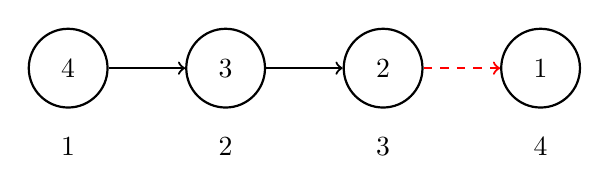
\begin{tikzpicture}[thick]
        \edef\pos{0}
        \foreach \x in {1, 2,..., 4}{
            \pgfmathparse{\pos+2}
            \xdef\pos{\pgfmathresult}
            \node  at (\pos, -1) {$\x$};
        }
        \node[circle,draw, minimum size=1cm] (1) at  (2, 0) {$4$};
        \node[circle,draw, minimum size=1cm] (2) at  (4, 0) {$3$};
        \node[circle,draw, minimum size=1cm] (3) at  (6, 0) {$2$};
        \node[circle,draw, minimum size=1cm] (4) at  (8, 0) {$1$};
        \draw[->] (1) -- (2);
        \draw[->] (2) -- (3);
        \draw[->, color=red, dashed] (3) -- (4);
    \end{tikzpicture}
    \caption[Exemplo de expiração de certificado da lista ordenada]{No exemplo da
    Figura~\ref{fig:ordenacao:exemplo}, \cert[3] expirou no instante $t = 2$.}
    \label{fig:lista:expire}
\end{figure}

Um evento está associado a um par $(e, t)$ que corresponde ao
certificado do elemento $e$ que expira no instante $t$, veja a Figura~\ref{fig:abb:expire}.
O tratamento do evento correspondente a esse par $(e, t)$ consiste em trocar de
lugar o elemento $e$ e seu predecessor, digamos $e'$, na árvore
binária de busca e na lista ligada, e recalcular o prazo de validade
de até três certificados, ilustrado na Figura~\ref{fig:abb:after}:

\begin{itemize}
    \item do certificado de $e$;
    \item do certificado de $e'$;
    \item do certificado do novo sucessor de $e'$, caso não seja \textsc{null}.
\end{itemize}

\begin{figure}
    \centering
    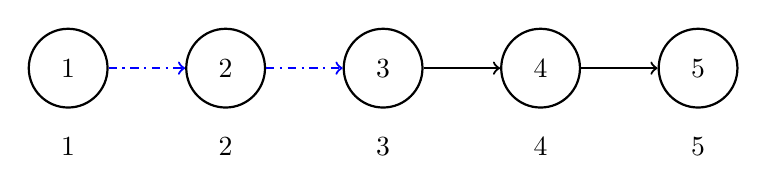
\begin{tikzpicture}[thick]
        \edef\pos{0}
        \foreach \x in {1, 2,..., 5}{
            \pgfmathparse{\pos+2}
            \xdef\pos{\pgfmathresult}
            \node[circle,draw, minimum size=1cm] (\x) at
                (\pos, 0) {$\x$};
            \node  at (\pos, -1) {$\x$};
        }
        % \foreach \x [evaluate=\x as \y using int(\x + 1)] in {1, 2,..., 4}{
        %     \ifthenelse{\x==2}{\draw[->, draw=red] (\x) -- (\y);}{\draw[->, draw=black] (\x) -- (\y);}
        % }
        \draw[->, color=blue, dashdotted] (1) -- (2);
        \draw[->, color=blue, dashdotted] (2) -- (3);
        \draw[->] (3) -- (4);
        \draw[->] (4) -- (5);
        % \draw[->] (1) edge (2) (2) edge (3) (3) edge (4) (4) edge (5)
    \end{tikzpicture}
    \caption[Certificados atualizados]{Após a mudança de velocidade
            do elemento 2, que se encontra em \sorted[2], \cert[1] e
            \cert[2] foram atualizados.}
    \label{fig:lista:after}
\end{figure}

Na implementação da operação \textsc{event}, no Algoritmo~\ref{alg:abb:evento}, utilizaremos a rotina
$\textsc{update}(e)$, no Algoritmo~\ref{alg:abb:update}, que calcula o novo prazo de validade $t$
do certificado do elemento $e$, e chama a rotina~$\textsc{updatePQ}(Q, e, t)$.
A função $\textsc{swap}(e_1, e_2)$ troca a posição de $e_1$ e $e_2$ na árvore binária balanceada
de busca e na lista ligada e a função \Call{expire}{$e,e'$} calcula
a validade do certificado entre os elementos $e$ e $e'$; se $e'$ é
\textsc{null}, retorna $+\infty$.

\begin{algorithm}[H]
    \caption{Função \textsc{update}.} \label{torneioi:update}
    \begin{algorithmic}[1]
        \Function{update}{$e$}
            \If{$e \neq$ NULL}
                \State $e'\leftarrow \torneio[(e.\lastmatch)/2]$
                \State $t \leftarrow $ \Call{expire}{$e, e'$}
                \State \Call{updatePQ}{$Q,e,t$}
            \EndIf
        \EndFunction
        % \LineComment{Em expire$(e, e')$, $e'$ pode ser nulo e
        % nesse caso o retorno é $+\infty$.}
        % \LineComment{\Call{expire}{$e,e'$} calcula a validade do
        % certificado entre os elementos $e$ e $e'$, se $e'$ é NULL
        % retorna $+\infty$}
    \end{algorithmic}
\end{algorithm}

\begin{algorithm}[H]
    \caption{Função \textsc{event}.} \label{torneioi:evento}
    \begin{algorithmic}[1]
        \Function{event}{\nnull}
            \State $e \leftarrow  $ \Call{minPQ}{$Q$}
            \While{$e.\cert$ = \now}
                \State $j \leftarrow e.\lastmatch$
                \State $k \leftarrow 2\cdot \floor{\frac{j}{2}}
                + ((j + 1)\mod2)$ \Comment{adversário}
                \While{$j > 1$ \AND \Call{value}{$j$} $\geq$
                    \Call{value}{$k$}}
                    \State \torneio[$\floor{\frac{j}{2}}$]
                    $\leftarrow~$\torneio[$j$]
                    \State $\torneio[k].\lastmatch$ $\leftarrow k$
                    \State \Call{update}{$\torneio[k]$}
                    \State $j \leftarrow \floor{\frac{j}{2}}$
                    \State $k \leftarrow 2\cdot \floor{\frac{j}{2}}
                    + ((j + 1)\mod2)$ \Comment{adversário}
                \EndWhile
                \State $\torneio[j].\lastmatch \leftarrow j$
                \State \Call{update}{$\torneio[j]$}
                \State $e \leftarrow  $ \Call{minPQ}{$Q$}
            \EndWhile
        % \LineComment{swapHeap$(i, \floor{\frac{i}{2}})$ troca \heap[$i$] por \heap$\left[\floor{\frac{i}{2}}\right]$}
        \EndFunction
%        \LineComment{\Call{compare}{$i, j$} retorna se o valor
%        de $i$ é maior que o valor de $j$.}
    \end{algorithmic}
\end{algorithm}

A operação \textsc{query\_kth}$(i)$ consiste em devolver o $i$-ésimo
maior elemento da lista ligada, ou seja, o $i$-ésimo da direita para
a esquerda, pois a árvore está em ordem crescente da esquerda para a
direita.
Para tal, percorreremos a árvore binária balanceada de busca utilizando o atributo $\children$
para, a cada iteração, decidir em qual subárvore o $i$-ésimo está, ajustando $i$ quando
necessário.
O Algoritmo~\ref{alg:abb:query} implementa esta operação e a Figura~\ref{fig:abb:queryexecution}
simula a execução em um exemplo.
A rotina auxiliar \textsc{rsize}$(r)$ devolve o valor de $r.\dir.\textit{size}$ caso $r.\dir$ seja
não nulo, caso contrário devolve $0$.

\input{conteudo/capitulos/ordenacao/figuras/abb/query_structure}

\begin{figure}
    \centering
    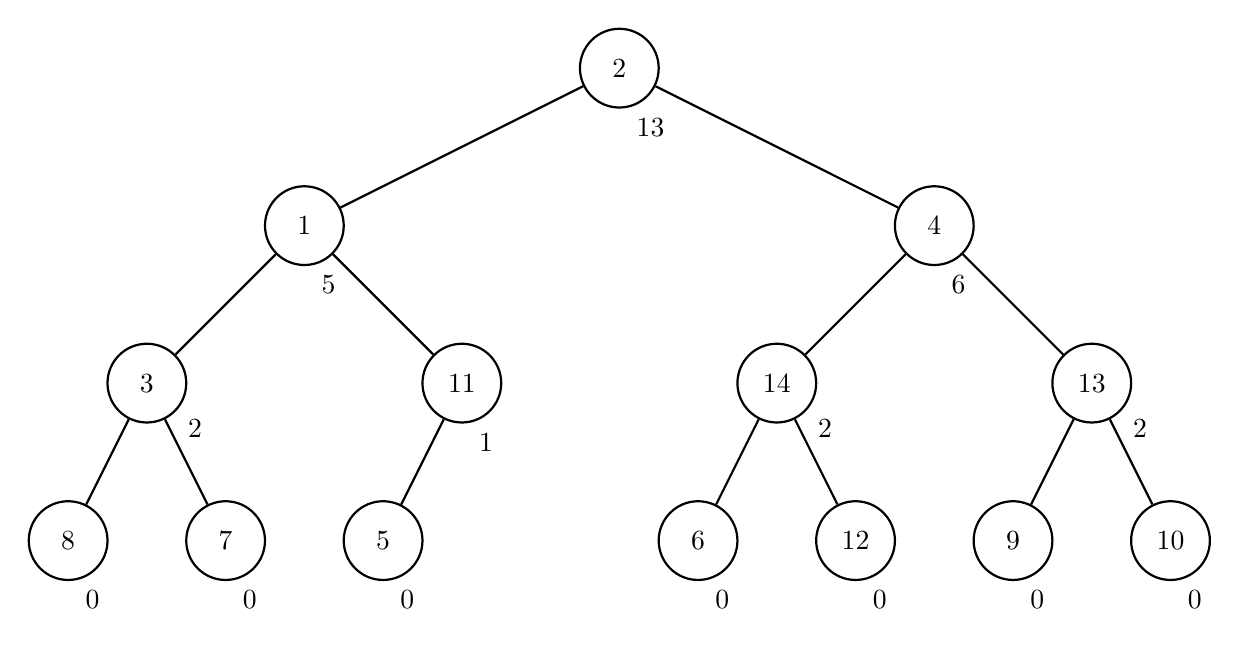
\begin{tikzpicture}[thick]
        \node[label=280:{13},circle,draw,minimum size=1cm]
            (1) at (0,0) {$2$};
        \node[label=280:{5},circle,draw,minimum size=1cm]
            (2) at (-4,-2) {$1$};
        \node[label=280:{6},circle,draw,minimum size=1cm]
            (3) at (4,-2) {$4$};
        \node[label=320:{2},circle,draw,minimum size=1cm]
            (4) at (-6,-4) {$3$};
        \node[label=280:{1},circle,draw,minimum size=1cm]
            (5) at (-2,-4) {$11$};
        \node[label=320:{2},circle,draw,minimum size=1cm]
            (6) at (2,-4) {$14$};
        \node[label=320:{2},circle,draw,minimum size=1cm]
            (7) at (6,-4) {$13$};
        \node[label=280:{0},circle,draw,minimum size=1cm]
            (8) at (-7,-6) {$8$};
        \node[label=280:{0},circle,draw,minimum size=1cm]
            (9) at (-5,-6) {$7$};
        \node[label=280:{0},circle,draw,minimum size=1cm]
            (10) at (-3,-6) {$5$};
        % \node[label={11},circle,draw,minimum size=1cm] (11) at (-1,-6) {$3$};
        \node[label=280:{0},circle,draw,minimum size=1cm]
            (12) at (1,-6) {$6$};
        \node[label=280:{0},circle,draw,minimum size=1cm]
            (13) at (3,-6) {$12$};
        \node[label=280:{0},circle,draw,minimum size=1cm]
            (14) at (5,-6) {$9$};
        \node[label=280:{0},circle,draw,minimum size=1cm]
            (15) at (7,-6) {$10$};

        \draw[thick] (1) -- (2);
        \draw[thick] (2) -- (4);
        \draw[thick] (4) -- (8);
        \draw[thick] (4) -- (9);
        \draw[thick] (2) -- (5);
        \draw[thick] (5) -- (10);
        % \draw[thick] (5) -- (11);
        \draw[thick] (1) -- (3);
        \draw[thick] (3) -- (6);
        \draw[thick] (3) -- (7);
        \draw[thick] (6) -- (12);
        \draw[thick] (6) -- (13);
        \draw[thick] (7) -- (14);
        \draw[thick] (7) -- (15);
    \end{tikzpicture}
    \caption[Como buscar $i$-ésimo na ABB]{Se quiséssemos encontrar
            o $7^\circ$ elemento na árvore acima, $i = 7$, desviamos
            para a direita, pois a quantidade de nós da subárvore
            direita da raiz é $\leq i$. Depois, desviamos para a
            esquerda e redefinimos $i$ como $3$, pois existem $4$
            elementos à frente. Como o nó do elemento $14$ só tem um
            nó em sua subárvore direita, desviamos para a esquerda
            de novo e redefinimos $i$ como $1$. Como a quantidade de
            nós da subárvore direita do nó do elemento $6$  somada a
            $1$ é igual a $i$, o elemento $6$ é o $7^\circ$ elemento
            da coleção.}
    \label{fig:abb:query}
\end{figure}

\begin{algorithm}
    \caption{Função \textsc{query\_kth}.} \label{abb:query}
\begin{algorithmic}[1]
    \Function{query\_kth}{$i$}
        \State $node \leftarrow root$
        \State $r \leftarrow \Call{rsize}{node}$
        \While{$i \neq r + 1$}
        \If{$i \leq r$}
            \State $node \leftarrow node.right$
        \Else
            \State $node \leftarrow node.left$
            \State $i \leftarrow i - (r + 1)$
        \EndIf
        \State $r \leftarrow \Call{rsize}{node}$
        \EndWhile
        \State \Return $node.key$
    \EndFunction
\end{algorithmic}
\end{algorithm}

A operação \textsc{change}$(j, v)$, como implementada no Algoritmo~\ref{alg:abb:change}, consiste em
recuperar o elemento $e$ com identificador $j$, alterar seu atributo \initv~para $x_0 +
(\speed - v)\cdot now$, \textit{speed} para \textit{v} e
recalcular os eventuais certificados de que $j$ participa, que
seriam $e.cert$ e $e.next.cert$, se $e.next$ existe.
A Figura~\ref{fig:abb:change} ilustra um exemplo com os elementos afetados.

\begin{algorithm}
    \caption{Função \textsc{change}.} \label{lista:change}
\begin{algorithmic}[1]
    \Function{change}{$j, v$}
        \State $x_0$[$j$] $\leftarrow  x_0$[$j$]
        $+~($\speed[$j$]$~-~v)~\cdot~$\now;
        \State \speed[$j$] $\leftarrow  v$
        \State $i \leftarrow$ \inds[$j$]
        \State \Call{update}{$i$}
        \State \Call{update}{$i - 1$}
    \EndFunction
\end{algorithmic}
\end{algorithm}

\begin{algorithm}
    \caption{Função \textsc{change}.} \label{lista:change}
\begin{algorithmic}[1]
    \Function{change}{$j, v$}
        \State $x_0$[$j$] $\leftarrow  x_0$[$j$]
        $+~($\speed[$j$]$~-~v)~\cdot~$\now;
        \State \speed[$j$] $\leftarrow  v$
        \State $i \leftarrow$ \inds[$j$]
        \State \Call{update}{$i$}
        \State \Call{update}{$i - 1$}
    \EndFunction
\end{algorithmic}
\end{algorithm}

A operação \textsc{insert}$(v, x_t)$, como ilustrado na Figura~\ref{fig:abb:insert}, consiste em
criar um novo elemento, inicializando seus atributos com os devidos valores, inseri-lo na
árvore binária balanceada de busca e na estrutura que usamos para
recuperá-lo depois, calcular o seu certificado e inseri-lo na fila
com prioridades e, por fim, atualizar o certificado de seu sucessor,
caso exista.
Uma importante observação é que se \now~$\neq 0$, então $x_t \neq$~\initv.
Para calcular \initv, podemos utilizar a relação
${x_t = now\cdot \speed + x_0}$, que implica que ${x_0 = x_t -
\speed\cdot now}$.
O Algoritmo~\ref{alg:abb:insert} implementa esta operação.

\begin{algorithm}
    \caption{Função \textsc{insert}.} \label{torneioi:insert}
    \begin{algorithmic}[1]
        \Function{insert}{$v, x_t$}
            \State $e.speed \leftarrow v$
            \State $e.x_0 \leftarrow x_t - now\cdot v$
            \State \raiz~$\leftarrow$ \Call{insertObject}{$root, e$}
            \State \Call{insertTourn}{$e$}
            \State \Call{newCert}{$e$}
            \State \Call{insertPQ}{$Q, e$}
        \EndFunction
    \end{algorithmic}
\end{algorithm}

\begin{algorithm}
    \caption{Função \textsc{insert}.} \label{torneioi:insert}
    \begin{algorithmic}[1]
        \Function{insert}{$v, x_t$}
            \State $e.speed \leftarrow v$
            \State $e.x_0 \leftarrow x_t - now\cdot v$
            \State \raiz~$\leftarrow$ \Call{insertObject}{$root, e$}
            \State \Call{insertTourn}{$e$}
            \State \Call{newCert}{$e$}
            \State \Call{insertPQ}{$Q, e$}
        \EndFunction
    \end{algorithmic}
\end{algorithm}

A operação \textsc{delete}$(i)$ consiste em recuperar o elemento
$i$, removê-lo da árvore binária balanceada de busca e da estrutura
que usamos para recuperá-lo, e depois removê-lo da fila com
prioridades.
Após isso, basta atualizar o certificado de seu sucessor, caso exista.
Essa operação é ilustrada na Figura~\ref{fig:abb:delete} e implementada no
Algoritmo~\ref{alg:abb:delete}.

\begin{algorithm}
    \caption[Algoritmo \textsc{delete} da árvore binária de busca]{Função \textsc{delete}.} \label{alg:abb:delete}
    \begin{algorithmic}[1]
        \Function{delete}{$i$}
            \State $e \leftarrow$ \Call{getObject}{$i$}
            \State $e' \leftarrow e.next$
            \State \raiz~$\leftarrow$ \Call{deleteKey}{$\raiz, e$}
            \State \Call{deleteObject}{$e$}
            \State \Call{deletePQ}{$Q, e$}
            \State \Call{update}{$e'$}
        \EndFunction
    \end{algorithmic}
\end{algorithm}

\begin{algorithm}
    \caption[Algoritmo \textsc{delete} da árvore binária de busca]{Função \textsc{delete}.} \label{alg:abb:delete}
    \begin{algorithmic}[1]
        \Function{delete}{$i$}
            \State $e \leftarrow$ \Call{getObject}{$i$}
            \State $e' \leftarrow e.next$
            \State \raiz~$\leftarrow$ \Call{deleteKey}{$\raiz, e$}
            \State \Call{deleteObject}{$e$}
            \State \Call{deletePQ}{$Q, e$}
            \State \Call{update}{$e'$}
        \EndFunction
    \end{algorithmic}
\end{algorithm}

\FloatBarrier

\subsection{Análise de desempenho}\label{subsec:analise-de-desempenho-abb}

A árvore binária balanceada de busca é uma estrutura \textit{responsiva}, pois o
custo de processar um certificado é $O(\lg{n})$, onde $n$ é o número de elementos sendo mantidos.
O custo de processar um certificado corresponde a uma iteração da linha $3$ na operação
\textsc{event}, que atualiza a posição dos elementos na árvore em $O(1)$ e realiza alterações na
fila de certificados em tempo $O(\lg{n})$, por isso o custo total de $O(\lg{n})$
para processar um certificado.

Assim como a lista ordenada cinética, a árvore binária balanceada de busca é uma
estrutura \textit{eficiente}, \textit{compacta} e \textit{local}, pelas mesmas
justificativas já apresentadas na seção da lista ordenada cinética.

Apesar do mesmo bom desempenho que a lista ordenada cinética, a árvore de busca
binária balanceada realiza a operação \textsc{query-kth} em $O(\lg{n})$, que é um
desempenho assintótico pior em relação a lista ordenada cinética, que realiza a
mesma operação em $O(1)$.

O desempenho pior na operação \textsc{query-kth} é justificado pelo ganho de
desempenho nas operações \textsc{insert} e \textsc{delete} que também são
realizadas em tempo $O(\lg{n})$, enquanto que na lista ordenada cinética o tempo
gasto é $O(n)$, pois precisamos mover $O(n)$ objetos para posicionar o novo
objeto na posição correta ou para reorganizar o vetor de forma a ocupar a
posição que ficou vazia após a remoção de um objeto.
